\section{Rivers \& Streams}

Essential to the realism of virtual rural terrains are water networks which take the form of rivers and streams. These rivers form as run-off water is being transported by gravity from higher to lower grounds. In this section is  The algorithm used to model gravity and therefore the evacuation of water on any terrain is outlined below along with details on the GPU implementation used to accelerate the process.

\subsection{Water Evacuation Algorithm} 

Precipitation, precipitation intensity and soil infiltration are used to calculate the soil humidity, $S_{h}$, which equates to the quantity of water, in millimetres, absorbed by the soil. The standing water, \textit{W$_{standing}$}, equated to the quantity of water which wasn't absorbed by the soil. It can be calculated using equation \ref{eq:standing_water_calculation}.

\begin{equation} \label{eq:standing_water_calculation}
	W_{standing} = R_{q} - S_{h}
\end{equation}
where:
\begin{itemize}
\item \textit{W$_{standing}$} is the standing water, in millimetres.\\
\item \textit{R$_{q}$} is the monthly rainfall quantity, in millimetres.\\
\item \textit{S$_{h}$} is the quantity of water absorbed by the soil, in millimetres.\\
\end{itemize}

Given the quantity of standing water, W$_{standing}$, for each vertex, a hydrostatic pipe-model similar to that of Stava et al. \cite{StAva2008} is used to determine the movement and build-up of water on the terrain. The hydrostatic pipe-model works by iteratively attempting to evacuate water from each vertex \textit{V} to any of it's eight surrounding vertices.\\

Although the algorithm is implemented to work in three dimensions where each vertex can evacuate water content to 8 surrounding vertices, it also works in a two-dimensional space. With this reduced dimensionality, each vertex \textit{V$_{n}$} has only two surrounding vertices (\textit{V$_{n-1}$} and \textit{V$_{n+1}$) in which water can be placed. To simplify the description of this algorithm, it will be described for two dimensions. \\

The following abbreviations will be used in this section:
\begin{itemize}
\item \textit{TerrainHeight$_{n}$}: The terrain height at vertex \textit{V$_{n}$}.
\item \textit{WaterHeight$_{n}$}: The water height at vertex \textit{V$_{n}$}.
\item \textit{AggregateHeight$_{n}$ = TerrainHeight$_{n}$ + WaterHeight$_{n}$}.
\end{itemize}

Depending on the water evacuation capacity, \textit{WEC} (see \ref{eq:water_evacuation_capacity}), of vertex V$_{n}$, one of three scenarios can occur: \textit{all water can be evacuated}, \textit{a portion of the water can be evacuated} and \textit{no water can be evacuated}. Each scenario is treated separately below.\\

\begin{equation} \label{eq:water_evacuation_capacity}
	WEC = 2 \times TerrainHeight_{n} - AggregateHeight_{n-1} - AggregateHeight_{n+1} > WaterHeight_{n}
\end{equation}

\textbf{ALL WATER CAN BE EVACUATED}\\

This holds true when:

\begin{equation}
	WEC >= WaterHeight_{n}
\end{equation}

In this situation, water is split to surrounding vertices proportionally to their height. This is to model the fact that water flows more intensely on steeper slopes. The quantity of water \textit{W$_{n-1}$} and \textit{W$_{n+1}$} to be placed on vertices \textit{V$_{n-1}$} and \textit{V$_{n+1}$} respectively is calculated as follows:

\begin{equation}
\textit{W_{n-1}} = \frac{TerrainHeight_{n} - AggregateHeight_{n-1}}{WEC} \times WaterHeight_{n}
\end{equation}

\begin{equation}
\textit{W_{n+1}} = \frac{TerrainHeight_{n} - AggregateHeight_{n+1}}{WEC} \times WaterHeight_{n}
\end{equation}

Examples such situations are illustrated in figure \ref{fig:evacuation_all}.

\begin{figure}
\center
	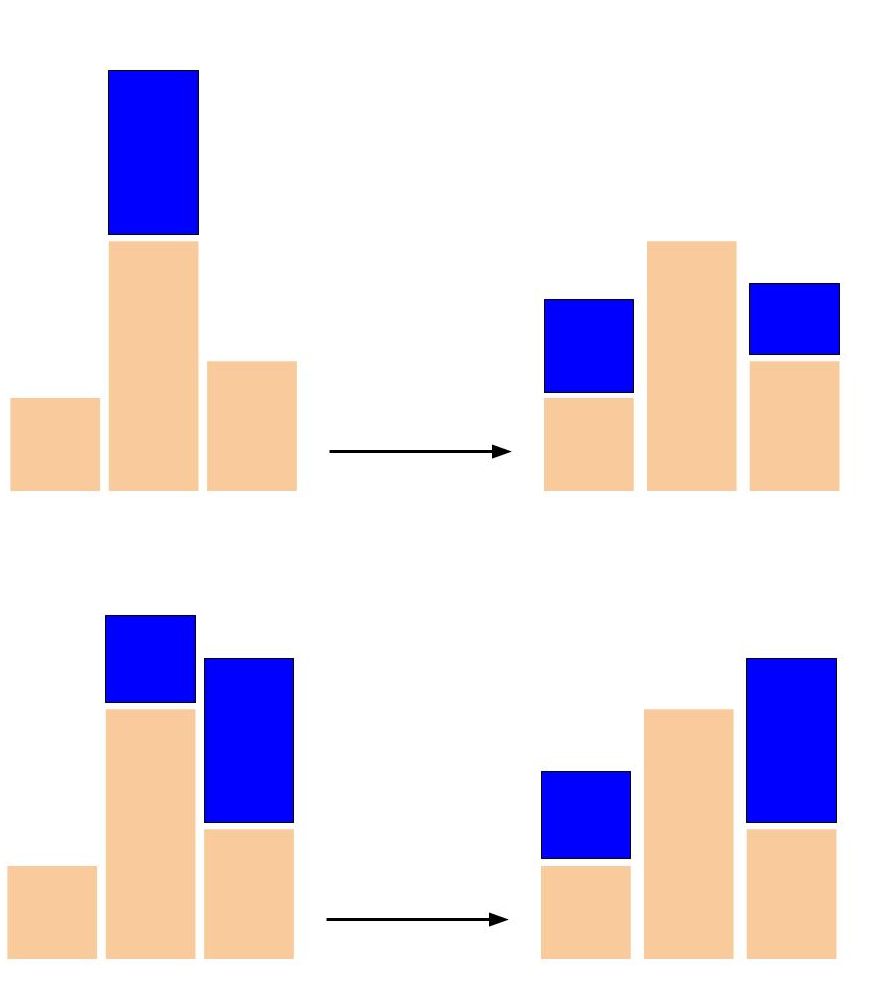
\includegraphics[width=\textwidth]{water_evacuation_all.png}
	\caption{ Example water evacuation scenarios where all water can be evacuated from source vertex (middle).}
	\label{fig:evacuation_all}
\end{figure}

\textbf{A PORTION OF THE WATER CAN BE EVACUATED}\\

This scenario occurs when the following holds true:

\begin{equation}
	0 < WEC < WaterHeight_{n}
\end{equation}

The portion of water which can be evacuate, \textit{W$_{evacuate}$} is calculated using \ref{eq:evacuate_calc}. 

\begin{equation}\label{eq:evacuate_calc}
	W_{evacuate} = AggregateHeight_{n} - W_{level}
\end{equation}

Where:
\begin{itemize}
 \item W$_{level}$ is the water level to which water must be evacuated (see \ref{eq:water_level_calc}).
\end{itemize}

\begin{equation} \label{eq:water_level_calc}
	W_{level} = \frac{AggregateHeight_{n-1} + AggregateHeight_{n} + AggregateHeight_{n+1}}{3}
\end{equation}

Examples such situations are illustrated in figure \ref{fig:evacuation_portion}.

\begin{figure}
\center
	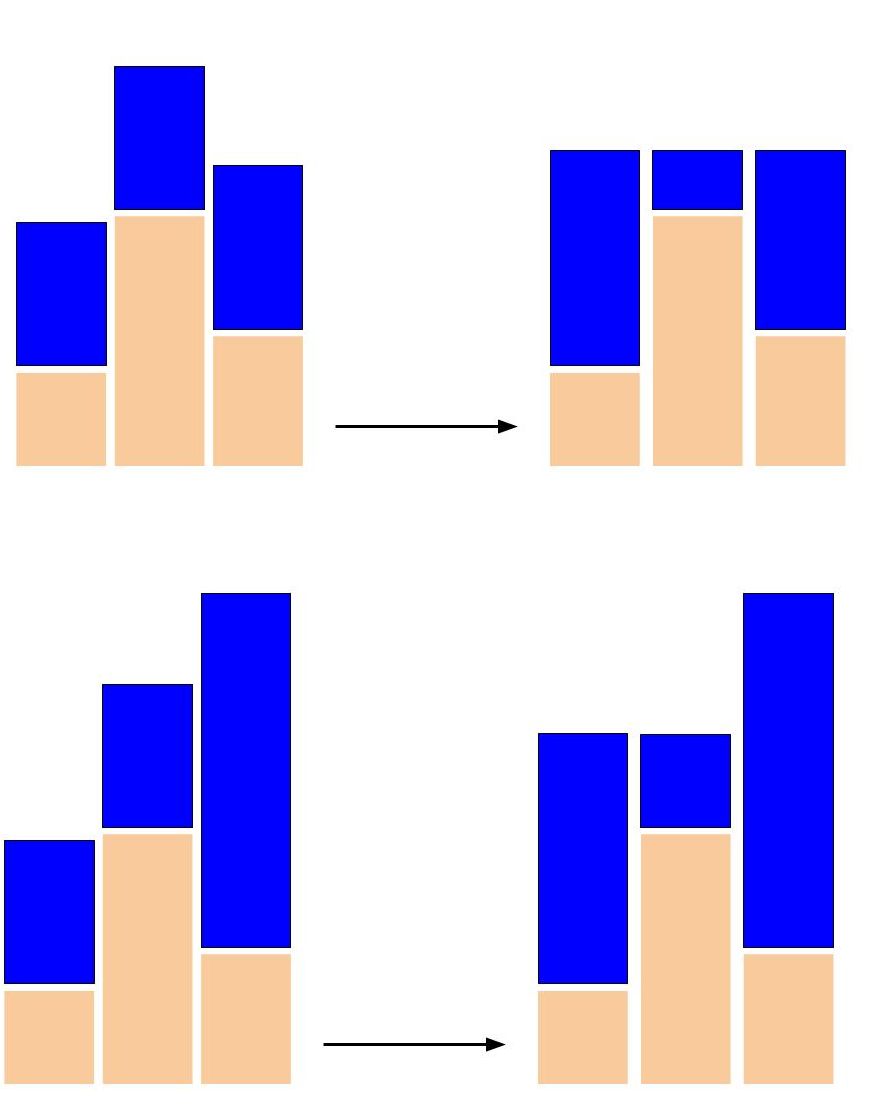
\includegraphics[width=\textwidth]{water_evacuation_portion.png}
	\caption{ Example water evacuation scenarios when only a portion of water can be evacuated from the source vertex (middle).}
	\label{fig:evacuation_portion}
\end{figure}

// Talk about terrain extremeties

Similarly to the work by , a water evacuation algorithm is used where water is iteratively evacuated from source to destination vertex. 

\subsection{GPU Implementation}

When processing a single vertex, water can not be removed from surrounding vertices

Both the standing water and the water evacuation algorithm was implemented on the GPU

through the evacuation of run-off water from higher to lower altitudes and, eventually, 

Water networks form due to the evacuation of 
